\ProvidesFile{ch-simulation.tex}[Light Curve Simulation]

\chapter{Light Curve Simulation}

Light curve simulation and inversion requires background knowledge in attitude kinematics, time and coordinate systems, computer graphics, and photometry.

\section{Attitude}

In order to effectively compute reflections and shadows on the surfaces of space objects, that object must have an assigned orientation in inertial space. While defunct satellites and space debris are slowly spun up by the Yarkovsky-O'Keefe-Radzievskii-Paddack (YORP) effect, the short-term motion of non-operational space objects is well-approximated by torque-free motion \cite{benson2018cyclic}. Developing the kinematics of torque-free motion first requires an understanding of common kinematic representations of orientation.

\subsection{Attitude Representations}

When discussing about the orientation of a rigid body in three dimensions, otherwise known as its attitude, that orientation is implicitly understood to be relative to some other reference frame. The direction of a unit vector can be expressed with two numbers ---  the azimuth and elevation of that vector. Naïvely, this could be extrapolated to conclude that six numbers are needed to express an orientation. Because the basis vectors form an orthonormal set $\left\{ \hat{b}_1, \hat{b}_2, \hat{b}_3\right\}$, it follows for a right-handed system that $\hat{b}_3 = \hat{b}_1 \times \hat{b}_2$, $\hat{b}_2 = \hat{b}_3 \times \hat{b}_1$, and $\hat{b}_1 = \hat{b}_2 \times \hat{b}_3$. Each of these equations constrains one further degree of freedom, revealing that a minimum of three quantities are necessary to express the relative orientation of two reference frames. This minimum bound does not make any statements about the usefulness of three element sets; at least four dimensions are needed to remove singularities. 

\subsubsection{The Direction Cosine Matrix}

The direction cosine matrix (DCM) is a $3\times3$ symmetric, orthogonal matrix, expressing the three basis vectors of one frame in another. This amounts to projecting each basis vector in the initial frame onto each basis vector of the final frame; the cosine of the angle between the compared vectors. It is notated with two capital letters, the rightmost indicating the reference frame of the input vectors and the leftmost indicating the transformed frame. Alternatively, the DCM is sometimes expressed as $C$ when the frames involved are arbitrary or do not need to be denoted. For example, the DCM $\dcm{bn}$ takes a vector $\vrf{n}{r}$ in the $\rf{n}$ frame to the $\rf{b}$ frame as $\vrf{b}{r}$:

\begin{equation}
    \vrf{b}{r} = \dcm{bn} \vrf{n}{r}.
\end{equation}

The orthogonal property of the DCM implies $\dcm{bn}^{-1} = \dcm{bn}^T$ such that $\dcm{bn}^T = \dcm{nb}$. 

\subsubsection{Principal Rotation Parameters}

Another common attitude representation is the Euler angle-axis set, otherwise known as principal rotation parameters \cite{crassidis1ed}. Euler's rotation theorem guarantees that any relative orientation can be expressed as a single rotation about an axis $\hat{\lambda} \in \mathbb{S}^2$ by an angle $\theta \in [0, 2\pi]$ \cite{crassidis1ed}. The set $\left\{\hat{\lambda},\theta\right\}$ is known as a principal rotation parameter, abbreviated PRP hereafter. The DCM is mapped to the PRP representation with:

\begin{align*} \numberthis \labelAndRemember{eq:dcm_to_prp}
    {
    \theta &= \cos^{-1}\left(\frac{1}{2} \left[C_{1,1} + C_{2,2} + C_{3,3} - 1 \right] \right), \\
    \hat{\lambda} &= \frac{1}{2\sin{\theta}} 
    \begin{bmatrix} C_{2,3} - C_{3,2} \\ C_{3,1}-C_{1,3} \\ C_{1,2} - C_{2,1}\end{bmatrix},
    }
\end{align*}

where $C_{i,j}$ refers to the $i$th row and $j$th column of $C$ \cite{shuster1993}. The mapping from PRP to DCM is also relatively straightforward:

\begin{equation} \labelAndRemember{eq:prp2dcm}
    {C = I_3 + \sin\theta\matcp{\hat{\lambda}} + (1-\cos\theta)\matcp{\hat{\lambda}}^2,}
\end{equation}

were $\matcp{v}$ is the matrix cross product operator, defined on $\vctr{v} \in \mathbb{R}^3$ as:

\begin{equation}
    \matcp{\vctr{v}} = \begin{bmatrix}
        0 & -v_3 & v_2 \\
        v_3 & 0 & -v_1 \\
        -v_2 & v_1 & 0
    \end{bmatrix}.
\end{equation}

This operator is useful as it rephrases the cross product as matrix multiplication, i.e. $\vctr{v} \times \vctr{u} = \matcp{\vctr{v}}\vctr{u}$. While the PRP $\{\theta, \hat{\lambda}\}$ is a four element set, there are only three degrees of freedom due to the unit norm constraint on $\hat{\lambda}$. 

\subsubsection{Quaternions}

The quaternion represents attitude with a point on the surface of the hypersphere \sthree. In terms of the PRP, the quaternion is given by \cite{crassidis1ed}:

\begin{equation} \labelAndRemember{eq:prp2quat}
    {
    \vctr{q} = \begin{bmatrix} \hat{\lambda} \sin\left( \theta \right) \\ \cos(\theta) \end{bmatrix}.
    }
\end{equation}

The first three entries of the quaternion are often called the vector component, with the final entry being the scalar component. Some authors reorder the quaternion, placing the scalar term first. Often the entries of a single quaternion are referenced by index such that $\vctr{q} = \left[ q_1, q_2, q_3, q_4 \right]$. Similarly, the vector portion of the quaterion is referenced with $\vctr{q}_{1:3}$. The quaternion can be mapped back to the PRP \cite{crassidis1ed} via

\begin{align*} \numberthis \labelAndRemember{eq:quat2prp_theta} 
    {
    \theta &= \cos^{-1}\left(q_4 \right) \\
    \lambda &= \frac{\vctr{q}_{1:3}}{\sin{\theta}}.
    }
\end{align*}

The quaternion maps to the DCM \cite{crassidis1ed} via 

\begin{equation} \labelAndRemember{eq:quat2dcm}
    {
        C = \left[\begin{matrix}\ -\ q_2^2-\ q_3^2+q_1^2+q_4^2\ &\ 2\ q_1q_2+2\ q_3q_4&\ 2\ q_1q_3-2\ q_2q_4\\\ 2\ q_1q_2-2\ q_3q_4&\ -\ q_1^2-\ q_3^2+q_2^2+q_4^2\ &\ 2\ q_1q_4+2\ q_2q_3\\\ 2\ q_1q_3+2\ q_2q_4&\ 2\ q_2q_3-2\ q_1q_4&\ -q_1^2-\ q_2^2+q_3^2+q_4^2\\\end{matrix}\right]=\Xi\left(q\right)^T\Psi\left(q\right).
    }
\end{equation}

In Eq \ref{eq:quat2dcm}, $\Psi$ is defined to be \cite{crassidis1ed}

\begin{equation} \label{eq:quat_psi}
    \Psi = \left[\begin{matrix}q_4&q_3&-q_2\\{-q}_3&q_4&q_1\\q_2&-q_1&q_4\\-q_1&-q_2&-q_3\\\end{matrix}\right].
\end{equation}

\subsection{Attitude Kinematics}

Because it is cheap to convert between attitude representations, only one set of kinematic equations are needed for propagating a rigid body attitude profile from an initial condition. Quaternion kinematic differential equations are chosen as they have no singularity and produce very smooth dynamics that are easy to integrate when compared to three-variable representations that possess singularities. Given the current orientation quaternion $\vctr{q} = [q_1, q_2, q_3, q_4]^T$ and angular velocity $\vctr{\omega} = [\omega_1, \omega_2, \omega_3]^T$ the quaternion derivative is computed via:

\begin{equation} \label{eq:quat_kde}
    \left[\begin{matrix}\dot{\epsilon_1}\\\dot{\epsilon_2}\\\dot{\epsilon_3}\\\dot{\epsilon_4}\\\end{matrix}\right]
    =
    \frac{1}{2}\left[\begin{matrix}\epsilon_4&-\epsilon_3&\epsilon_2&\epsilon_1\\\epsilon_3&\epsilon_4&-\epsilon_1&\epsilon_2\\-\epsilon_2&\epsilon_1&\epsilon_4&\epsilon_3\\-\epsilon_1&-\epsilon_2&-\epsilon_3&\epsilon_4\\\end{matrix}\right]
    \left[\begin{matrix}\omega_1\\\omega_2\\\omega_3\\0\\\end{matrix}\right].
\end{equation} 

\subsection{Attitude Dynamics}

Rigid body dynamics can be easily expressed in the body principal axes with an arbitrary torque $\vctr{M} = \left[M_1, M_2, M_3\right]^T$ in the same frame via:

\begin{equation} \label{eq:rbtf_dynamics}
    \left[\begin{matrix}\dot{\omega_1}\\\dot{\omega_2}\\\dot{\omega_3}\\\end{matrix}\right]
    =
    \left[\begin{matrix}
        \left(M_1+I_2\omega_2\omega_3-I_3\omega_2\omega_3\right) / I_1 \\
        \left(M_2-I_1\omega_1\omega_3+I_3\omega_1\omega_3\right) / I_2 \\
        \left(M_3+I_1\omega_1\omega_2-I_2\omega_1\omega_2\right) / I_3 \\
    \end{matrix}\right].
\end{equation}

Equations \ref{eq:rbtf_dynamics} and \ref{eq:quat_kde} are numerically integrated to yield the orientation time history which is necessary for later light curve simulations. Often, $\vctr{M} = \mathbf{0}$ is chosen to simulate the torque-free evolution of an initial orientation and spin state, neglecting small attitude perturbations over the simulation interval.

\graphicspath{{/Users/liamrobinson/Documents/PyLightCurves/docs/build/html/_images}}

\section{Computer Graphics}

The light curve simulation framework developed in this work relies on a pixel-by-pixel image rendering on the GPU to compute the total reflected irradiance at each timestep of the simulation. As a result, a background in common computer graphics terminology and reference frames is necessary to understand the transformation from coordinates in the object body frame to a pixel in the final image.

\subsubsection{Camera Projections and Terminology}

In computer graphics, a camera is defined by its position $R_{cam}$, target $T_{cam}$, reference up direction $U_{cam}$, and a field of view $FOV$. In order to render a 3D scene to a 2D image using this camera, a transformation is needed. An orthographic camera accomplishes this transformation by orthogonally projecting points onto a plane perpendicular to camera look direction $T_{cam} - R_{cam}$. The volume of space that falls into view of the camera is known as the frustum \cite{shirley2009}. An important consequence of orthogonal projection is that objects further away from the camera do not shrink in the image, which is sometimes advantageous. A perspective projection forms a more complex frustum that expands outwards from a near plane to a proportionally larger far plane. Because of the expansion of the frustum, geometry processed by the perspective transformation shrinks as it moves further from the near plane. Figure \ref{fig:ortho_perspective_cameras} displays the geometry of these camera frustums, with additional reference frames detailed in Section \ref{sec:graphics_trans}.

\begin{figure}[!htb]
  \centering
  \includegraphics[width=\figbig]{sphx_glr_computer_graphics_background_001.png}
  \caption{Perspective and orthographic projections with relevant camera frustum attributes labeled}
  \label{fig:ortho_perspective_cameras}
\end{figure}


\subsubsection{Transformations} \label{sec:graphics_trans}

Transformations in computer graphics are often represented by $4 \times 4$ matrices. These matrices operate on so-called homogeneous coordinates, operating on vectors in $\mathbb{R}^4$ of the form $\left[ x, y, z, w \right]^T$ \cite{shirley2009}. The inclusion of the fourth component enables simultaneous rotation, translation, and scaling of the input points by the matrix, provided that the outputs are normalized to set $w = 1$ \cite{shirley2009}.

There are a few fundamental matrices used in computer graphics that are necessary for later hardware-accelerated light curve simulation algorithms. The first is the model matrix $M \in \mathbb{R}^{4 \times 4}$ which transforms from the world frame to the model frame given the origin of the model body frame $R_{m} \in \mathbb{R}^{3 \times 3}$ and the orientation of the model body frame relative to the world frame $\mathbf{q}_m \in \mathbb{R}^4$ as a quaternion \cite{shirley2009}:

\begin{equation} \label{eq:model_matrix}
  M = \begin{bmatrix}
    -\ q_2^2-\ q_3^2+q_1^2+q_4^2\ &\ 2\ q_1q_2+2\ q_3q_4&\ 2\ q_1q_3-2\ q_2q_4 & -R_{m,x}\\
    \ 2\ q_1q_2-2\ q_3q_4&\ -\ q_1^2-\ q_3^2+q_2^2+q_4^2\ &\ 2\ q_1q_4+2\ q_2q_3 & -R_{m,y}\\
    \ 2\ q_1q_3+2\ q_2q_4&\ 2\ q_2q_3-2\ q_1q_4&\ -q_1^2-\ q_2^2+q_3^2+q_4^2 & -R_{m,z} \\
    0 & 0 & 0 & 1
  \end{bmatrix}.
\end{equation}

Eq \ref{eq:model_matrix} uses Eq \ref{eq:quat2dcm} to transform the quaternion into a DCM. The model matrix basis vectors are illustrated in Figure \ref{fig:ortho_perspective_cameras} as $M_i$, with the world frame basis vectors notated with $W_i$. Given the location of the camera origin $R_{cam} \in \mathbb{R}^3$, its target position $T_{cam} \in \mathbb{R}^3$, and the camera up direction $U_{cam} \in \mathbb{R}^3$, the view matrix $V \in \mathbb{R}^{4 \times 4}$ that transforms from the world frame to the camera frame is given by \cite{shirley2009}:

\begin{align*} \numberthis \label{eq:view_matrix}
  v_3 &= \frac{R_{cam} - T_{cam}}{\| R_{cam} - T_{cam} \|} \\
  v_1 &= \frac{U_{cam} \times v_z}{\| U_{cam} \times v_3 \|} \\
  v_2 &= v_1 \times v_3 \\
  V &= \begin{bmatrix}
    v_{1,x} & v_{1,y} & v_{1,z} & -v_1 \cdot R_{cam} \\
    v_{2,x} & v_{2,y} & v_{2,z} & -v_2 \cdot R_{cam} \\
    v_{3,x} & v_{3,y} & v_{3,z} & -v_3 \cdot R_{cam} \\
    0 & 0 & 0 & 1
  \end{bmatrix}.
\end{align*}

The view matrix basis vectors are illustrated in Figure \ref{fig:ortho_perspective_cameras} as $V_i$. Given the field of view of the camera $FOV$ in radians, the distance from the camera origin to the near $n$ and far $f$ clipping planes, and the camera aspect ratio $a$, the orthographic projection matrix $P \in \mathbb{R}^{4 \times 4}$ that transforms from the camera frame to the image plane is given by \cite{shirley2009}:

\begin{align*} \numberthis \label{eq:projection_matrix}
  t &= n \cdot \tan\left(\frac{FOV}{2}\right) \\
  r &= t \cdot a \\
  P &= \begin{bmatrix}
    \frac{2n}{2r} & 0 & 0 & 0 \\
    0 & \frac{2n}{2t} & 0 & 0 \\
    0 & 0 & - \frac{f+n}{f-n} & \frac{2fn}{f-n} \\
    0 & 0 & -1 & 0 \\
  \end{bmatrix}
\end{align*}

Together, these matrices form the so-called Model-View-Projection matrix which transforms directly from coordinates in the object body frame $r_{obj}$ to the image plane:

\begin{equation} \label{eq:mvp}
  \begin{bmatrix} x_h \\ y_h \\ z_h \\w_h \end{bmatrix} = M V P \begin{bmatrix} r_{obj,x} \\ r_{obj,y} \\ r_{obj,z} \\ 1 \end{bmatrix}.
\end{equation}

In Eq \ref{eq:mvp}, $x_h/w_h$ and $y_h/w_h$ are homogeneous coordinates in the image plane, running linearly from $[-1, -1]$ at the top left corner of the image to $[1, 1]$ at the bottom right. Given the width of the image in $w_{pix}$ pixels, the image coordinates $\left(x,y\right)$ of $r_{obj}$ in pixels are:

\begin{equation} \label{eq:homo_to_pix}
  \begin{bmatrix} x \\ y \end{bmatrix} = \begin{bmatrix} w_{pix} \left(\frac{1}{2} + \frac{x_h}{2w_h}\right) \\ a \cdot w_{pix}\left(\frac{1}{2} + \frac{y_h}{2w_h}\right) \end{bmatrix}.
\end{equation}

The transformation summarized in Eqs \ref{eq:mvp} and \ref{eq:homo_to_pix} are crucial in Section \ref{sec:shadow_mapping} for the shadow mapping algorithm used to compute pixel-wise self-shadowing effects.

\section{Time Systems}

In order to accurately predict the position of a space object and an observer, it is necessary to understand how a given time translates to the orientation of the relevant reference frames. These calculations require conversions between various time scales, the Julian date, and sidereal time.

\subsection{Time Scales}

There are a variety of scales used to measure time. What follows is a minimal treatment of each. For a more comprehensive overview, see Section 3.5 of \cite{vallado4ed}. International Atomic Time (TAI) is based on measurements from atomic clocks and is independent of astronomical effects or observations. By definition, TAI proceeds at the rate of $1$ SI second per second. Universal Time (UT0) is derived directly from observations of the apparent position of the stars. UT1 is derived from UT0 by adjusting for polar motion. UT1 is offset from TAI by $\Delta UT1$, which is a dynamic quantity that must be continually observed. Universal Coordinated Time (UTC) is a truncation of UT1 that uses an integer number of leap seconds $\Delta AT$ to stay within $0.9$ seconds of TAI. Terrestrial Time (TT) is defined by a constant offset of $TT - TAI = 32.184$ seconds from TAI and preceeding at the same rate as TAI. These time scale relations are summarized in Eq \ref{eq:time_scale_conversions}.

\begin{align*}  \label{eq:time_scale_conversions} \numberthis
  UTC &= UT1 - \Delta UT1 \\
  TAI &= UTC + \Delta AT \\
  TT &= TAI + 32.184^s \\
\end{align*}

These time scales are relevant for this research as the precise coordinate frame transformation from ITRF to the J2000.0 realization of ICRF relies on quanities expressed in UT1. Date timestamps are usually standardized to UTC, requiring the transformations in Eq \ref{eq:time_scale_conversions} for full accuracy. Figure \ref{fig:time_scales} shows the evolution of UTC, UT1, and TT with respect to TAI. Notice that $\Delta UT1$ continually changes while $\Delta AT$ is always truncated to a nearby integer.

\begin{figure}[ht]
  \centering
  \includegraphics[width=\figbig]{sphx_glr_time_systems_001.png}
  \caption{Time scales relative to TAI}
  \label{fig:time_scales}
\end{figure}

\subsection{Julian Date}

Most tasks in astrodynamics are easier when using a continuous time system. For this reason, the Julian date is adopted. This quantity is defined is the number of days elapsed since January 1, 4713 B.C., at 12:00 \cite{vallado4ed}. Given a date timestamp of the form D/M/Y h:m:s between the years of 1900 and 2100, the Julian date is computed via:

\begin{equation} \label{eq:date_to_jd}
  JD = 376Y - \fl{\left[ \frac{7Y + 7 \cdot \fl{\left(\frac{M + 9}{12} \right)}}{4} \right]}
      + \fl{\left(\frac{275M}{9}\right)} 
      + d
      + 1721013.5
      + \frac{\frac{\left(\frac{s}{60} + 60\right)}{60} + h}{24}.
\end{equation}

Note that Eq \ref{eq:date_to_jd} is always a function of the time scale used in the input, i.e., a UTC timestamp yields $JD_{UTC}$ whereas a UT1 timestamp yields $JD_{UT1}$. Another useful quantity for later time and coordinate system calculations is the number of Julian centuries since a particular epoch. The J2000.0 epoch is used unless otherwise stated, resulting in \cite{vallado4ed}:

\begin{equation} \label{eq:jd_to_t}
  T = \frac{JD - 2451545.0}{36535}.
\end{equation}

Often, more specificity is needed with respect to the time scale used in Eq \ref{eq:jd_to_t}. For example, computing $T$ with an input date in UT1 yields $T_{UT1}$ using $JD_{UT1}$, which is in turn a function a date timestamp expressed in UT1. 

\subsection{Solar and Sidereal Time}

A solar day is defined as the time required for the Sun to pass and return to an observer's meridian --- a line of constant longitude extending from the geographic south pole to the geographic north pole \cite{vallado4ed}. By contrast, a sidereal day is the time required for the stars to complete a revolution around an observer's meridian. Due to the Earth's orbit around the Sun, the sidereal day is about 4 minutes shorter than the solar day \cite{vallado4ed}. The Greenwich mean sidereal time (GMST) is computed in seconds via \cite{frueh2019notes}:

\begin{equation} \label{eq:date_to_gmst}
  \theta_{GMST} = 67310.54841
        + \left(3.15576 \cdot 10^9 + 8640184.812866 \right) T_{UT1}
        + 0.093104 T_{UT1}^2
        - 6.2 \cdot 10^{-6} T_{UT1}^3.
\end{equation}

Accounting for the variations in the inclination of the ecliptic $\epsilon$ and the the change in the equinox compared to the reference epoch $\Delta \Psi$ produces Greenwich apparent sidereal time (GAST) via \cite{frueh2019notes}:

\begin{equation} \label{eq:date_to_gast}
  \theta_{GAST} = \theta_{GMST} + \Delta \Psi \cos\epsilon.
\end{equation}

Both the inclination of the ecliptic and the difference in the equinox are computed with series expansions following the IAU 1980 theory of nutation \cite{vallado4ed}.

\section{Coordinate Systems}

A precise definition of coordinate systems is necessary for determining the position of the observer and the observed space object at a given time. The relevant conversions are summarized by a single question: how is a fixed position on the surface of the Earth transformed into a standardized inertial reference frame?

\subsection{Latitude, Longitude and Altitude}

Latitude, longitude, and altitude (LLA) are a spherical coordinates representation of position on or above the surface of the Earth. For the purposes of precise station positioning, the difference between the two types of longitude --- geocentric and geodetic --- is important. Geocentric latitude is the angle between the line from the center of mass of the Earth to the position of interest and the equatorial plane. Geodetic latitude instead measures the angle between the local ellipsoid surface normal and the equatorial plane. Geodetic latitude $\phi_{geod}$ is converted to geocentric $\phi_{geoc}$ latitude with \cite{frueh2019notes}:

\begin{equation} \label{eq:geod_to_geoc}
  \phi_{geoc} = \tan^{-1} \left((1 - f)^2 \tan\phi_{geod} \right).
\end{equation}

Additionally, the radius of the ellipsoid $r_E$ at a given geocentric latitude is necessary for later conversion, expressed by \cite{frueh2019notes}:

\begin{equation} \label{eq:rad_at_geoc}
  r_E = R_E - f \sin^2 \left( \phi_{geoc} \right).
\end{equation}

The altitude in an set of LLA coordinates needs a reference point. Different observers may be defined differently --- either relative to the approximate ellipsoidal shape of the Earth, the hypothetical mean sea level, or the surrounding terrain.

\subsubsection{Ellipsoid}

Due to Earth's equatorial bulge, it is common to model the rough shape of the Earth as an ellipsoid. In particular, the 1984 World Geodetic Survey (WGS-84) model is used throughout this work to define the shape of the Earth ellipsoid, with parameters listed in Table \ref{tb:wgs84} for use in Eqs \ref{eq:geod_to_geoc} and \ref{eq:rad_at_geoc}.

\begin{table}[ht]
  \centering
  \begin{tabular}{|l|l|}
  \hline
  \textbf{Parameter} & \textbf{Value}              \\ \hline
  Equatorial radius $R_E$             & $6378.137 \: [km]$ \\ \hline
  Flattening ratio $f$                & $1 / 298.257$      \\ \hline
  \end{tabular}
  \caption{WGS-84 ellipsoid model of the Earth \cite{vallado4ed}}
  \label{tb:wgs84}
\end{table}

These parameters are needed for the conversion from LLA to the International Terrestrial Reference Frame.

\subsubsection{Geoid}

The geoid accounts for the gravitational potential differences across the Earth's surface \cite{vallado4ed}. It is a surface of equal gravitational potential; the surface the ocean relaxes to without the influence of the wind and tides \cite{vallado4ed}. For this reason, the geoid is alternatively known as the mean sea level (MSL). The ellipsoid is a good approximation of the geoid, which deviates from the ellipsoid by less than $\approx 100$ meters at all latitudes and longitudes. The height of the geoid above the ellipsoid can be computed from a high-fidelity gravity model, but it is often more convenient to interpolate a pre-computed grid of geoid heights. Figure \ref{fig:geoid_shape} displays global geoid heights derived from the 1996 Earth Gravitational Model (EGM-96) relative to the ellipsoid.

\begin{figure}[ht]
  \centering
  \includegraphics[width=\figmed]{sphx_glr_geoid_heights_001_2_00x.png}
  \caption{EGM-96 geoid heights above the WGS-84 ellipsoid}
  \label{fig:geoid_shape}
\end{figure}

\subsubsection{Terrain}

Terrain elevation is usually the final component needed to fully define the altitude of a ground station, which is often defined relative to MSL. This work uses $30$-meter terrain tiles from the Shuttle Radar Topography Mission (SRTM). Figure \ref{fig:pogs_terrain} shows the local elevation around the Purdue Optical Ground Station using SRTM data.

\begin{figure}[ht]
  \centering
  \includegraphics[width=\figsmall]{sphx_glr_pogs_local_terrain_001.png}
  \caption{MSL elevations surrounding the Purdue Optical Ground Station}
  \label{fig:pogs_terrain}
\end{figure}

\subsubsection{Altitude Conversions}

Given an altitude relative to the terrain $a_{terrain}$, the elevation above the ellipsoid $a_{ellip}$ is given as a function of the terrain elevation above the geoid $h_{terrain}(\lambda, \phi)$ and the geoid elevation above the ellipsoid $h_{terrain}(\lambda, \phi)$ by:

\begin{equation} \label{eq:altitude_above_ellipsoid}
  a_{ellip} = a_{terrain} + h_{terrain}(\lambda, \phi_{geod}) + h_{geoid}(\lambda, \phi_{geod}).
\end{equation}

\subsection{International Terrestrial Reference Frame (ITRF)}

The cartesian form of LLA is known as the Earth-centered Earth-fixed (ECEF) reference frame. Throughout this work, ECEF and ITRF will be used interchangeably. This frame has its origin at the center of mass of the Earth and its axes fixed in the crust. The
fundamental plane of the frame is defined to be the equator ---  orienting the $z$-axis through Earth's
instantaneous spin axis, and the reference direction through the intersection of the prime meridian
and the equator ---  defining the $x$-axis. Completing the right-handed system with $\hat{y} = \hat{z} \times \hat{x}$ yields a
reference frame that remains fixed, neglecting effects like continental drift. The transformation from LLA $\left( \lambda, \phi_{geod}, a_{ellip} \right)$ to ITRF is given by Eq \ref{eq:lla_to_itrf}.

\begin{align*} \numberthis \label{eq:lla_to_itrf}
  e^2 &= 2f - f^2 \\
  N &= \frac{R_E}{\sqrt(1 - e^2 \sin(\phi_{geod})^2)} \\
  \rho &= (N + a_{ellip}) \cos(\phi_{geod}) \\
  x_{itrf} &= \rho \cos(\lambda) \\
  y_{itrf} &= \rho \sin(\lambda) \\
  z_{itrf} &= \left(N (1 - e^2) + a_{ellip} \right) \sin(\phi_{geod}) \\
\end{align*}

In Eq \ref{eq:lla_to_itrf}, $e^2$ is the squared eccentricity of the ellipsoid, $N$ is the radius of curvature in the meridian, and $\rho$ is the $x-y$ plane magnitude of the station's position \cite{vallado4ed}.

Many later transformations require the body axis rotation matrices $R_1$, $R_2$, and $R_3$ which are expressed in Eq \ref{eq:body_rotms}.

\begin{align*} \numberthis \label{eq:body_rotms}
  R_1(\theta) &= \begin{bmatrix}  1 & 0 & 0 \\ 0 & \cos\theta & \sin\theta \\ 0 & -\sin\theta & \cos\theta \end{bmatrix} \\
  R_2(\theta) &= \begin{bmatrix}  \cos\theta & 0 & -\sin\theta \\ 0 & 1 & 0 \\ \sin\theta & 0 & \cos\theta \end{bmatrix} \\
  R_3(\theta) &= \begin{bmatrix}  \cos\theta & \sin\theta & 0 \\ -\sin\theta & \cos\theta & 0 \\ 0 & 0 & 1 \end{bmatrix} \\
\end{align*}

\subsection{Topocentric Reference Frame (ENU)}

The remaining transformations in this chapter will only be defined in terms of their rotation matrices. It is often useful to express observations in a local reference frame. The East North Up (ENU) coordinate system is used throughout this work. This system has an origin at the observing station, with the first two basis vectors pointing towards the local East and North and the third pointing towards zenith. The transformation from ITRF to ENU is given by \cite{frueh2019notes}:

\begin{equation} \label{eq:itrf_to_enu}
  \vec{r}_{enu} = F_2 F_1 R_2(\phi_{geoc}) R_3(\lambda) \vec{r}_{itrf}.
\end{equation}

In Eq \ref{eq:itrf_to_enu}, $R_3$ is a rotation about the third body axis, $F_1$ swaps the second and third unit vectors, and $F_2$ swaps the first and third unit vectors. The orientation of the ENU reference frame at the Purdue Optical Ground Station is depicted in Figure \ref{fig:pogs_enu}.

\begin{figure}[ht]
  \centering
  \includegraphics[width=\figmed]{sphx_glr_az_el_parallel_001.png}
  \caption{ENU reference frame orientation at Purdue Optical Ground Station}
  \label{fig:pogs_enu}
\end{figure}

\subsection{International Celestial Reference Frame (ICRF/J2000)}

Transforming from ITRF to the a standardized intertial reference frame is an involved process due to the variety of nonlinear effects impacting the Earth's rotational motion. In total, this transformation must account for polar motion, the nutation and precession of the Earth's pole, and the mean sidereal time. These transformations are treated much more thoroughly in Vallado \cite{vallado4ed}. 

Accounting for polar motion --- the motion of the Earth's pole that cannot be explained through nutation theory --- transforms from ITRF to Greenwich True of Date (GTOD) via: 
\begin{equation} \label{eq:itrf_to_gtod}
  \vec{r}_{gtod} = R_1(y_p) R_2(x_p) \vec{r}_{itrf},
\end{equation}

where $x_p$ and $y_p$ are the angular components of the polar motion at the time of interest \cite{frueh2019notes}. Accounting for the sidereal rotation of the Earth about its pole transforms from GTOD to the True Equator, Mean Equinox (TEME) reference frame via \cite{frueh2019notes}:

\begin{equation} \label{eq:gtod_to_teme}
  \vec{r}_{teme} = R_3(-\theta_{GMST}) \vec{r}_{gtod}.
\end{equation}

Accounting for the difference between GMST and GAST at the date of interest transforms from TEME to the True of Date (TOD) reference frame via \cite{vallado4ed}:

\begin{equation} \label{eq:teme_to_tod}
  \vec{r}_{tod} = R_3(-\Delta \Psi \cos \epsilon) \vec{r}_{teme}.
\end{equation}

Accounting for the nutation of Earth's pole transforms from TOD to the Mean of Date (MOD) reference frame via:

\begin{equation} \label{eq:tod_to_mod}
  \vec{r}_{mod} = R_1(-\bar{\epsilon}) R_3(\Delta\Psi) R_1(\bar{\epsilon} + \Delta\epsilon) \vec{r}_{tod},
\end{equation}

where $\bar{\epsilon}$ is the mean inclination of the ecliptic at the time of interest, and $\epsilon$ is the true inclination of the ecliptic \cite{vallado4ed}.

Accounting for the secular precession of Earth's pole transforms from MOD to ICRF via:

\begin{equation} \label{eq:mod_to_icrf}
  \vec{r}_{icrd} = R_3(\zeta) R_2(\theta) R_3(z) \vec{r}_{mod},
\end{equation}

through the 3-2-3 Euler angle sequence $\left( z, \theta, \zeta \right)$, which are each a function of the date of the transformation \cite{frueh2019notes}.

The specific realization of ICRF used in this work is referenced to the position of the equator and equinox at the J2000.0 epoch (January 1, 2000 12:00:00.000 TT), leading to the common name for this reference frame, "J2000" \cite{vallado4ed}.

\subsection{Right Ascension and Declination}

Right ascension and declination, often shortened to RA/Dec, are useful angles from describing the angular position of an object on the celestial sphere from the perspective of an observer. Right ascension is defined as the angle
of the observation projected onto the inertial $x-y$ plane, measured counterclockwise from inertial
$\hat{x}$, represented by $\alpha$. Declination is the angle from the $x-y$ plane to the observation
with positive values above the $x-y$ plane (closer to inertial $z$) and negative values below.
Declination is represented by $\delta$. Given a unit vector direction $\hat{v} = \left[ x_{ITRF}, y_{ITRF}, z_{ITRF} \right]^T$ in J2000, RA/Dec is computed via \cite{frueh2019notes}:

\begin{equation} \label{eq:eci_to_ra_dec}
  \begin{bmatrix}
	\alpha \\
	\delta
  \end{bmatrix} = 
  \begin{bmatrix}
	\atantwo(y_{ITRF}, x_{ITRF}) \\
	\atantwo(z_{ITRF}, \sqrt{x_{ITRF}^2 + y_{ITRF}^2})
  \end{bmatrix}.
\end{equation}

\subsection{Azimuth and Elevation}

Azimuth and elevation, often shortened to Az/El, are similar angular quantities to right ascension and declination \cite{frueh2019notes}. Instead of being based on
the inertial sphere, they are referenced to an arbitrary reference frame. For a telescope making
observations of an object, the local topocentric ENU frame may be used. For a satellite star
tracker, star azimuth and elevation might be reported in the satellite body frame. In either case,
Eq \ref{eq:eci_to_ra_dec} can be repurposed in terms of Az/El, where $\hat{v} = \left[ x_{ENU}, y_{ENU}, z_{ENU}
\right]^T$ is expressed in the frame of interest \cite{frueh2019notes}.

\begin{equation} \label{eq:enu_to_az_el}
  \begin{bmatrix}
	Az \\
	El
  \end{bmatrix} = 
  \begin{bmatrix}
	\atantwo(y_{ENU}, x_{ENU}) \\
	\atantwo(z_{ENU}, \sqrt{x_{ENU}^2 + y_{ENU}^2})
  \end{bmatrix}
\end{equation}

Note that Eq \ref{eq:enu_to_az_el} references azimuth to the $x$-axis, proceeding in the
counterclockwise direction. Often, this reference axis and direction may be changed depending on the
reference frame being used. For example, ground station observations may be referenced to local
North ---  the second axis of the ENU system ---  proceeding clockwise. This would require the
substitution $Az' = \frac{\pi}{2} - Az$. Notice that this substitution leads to $Az'$ leaking
outside the domain of $[0, 2\pi)$. This is not an issue for later coordinate transformations, but
may be undesirable for plots. Wrapping the result back to the standard azimuth range via
$Az_{wrapped} = \textrm{mod}(Az, 2\pi)$ is a sufficient fix.

\subsection{Coordinate Transformations Summary}

With these transformations, any topocentric observation directions in RA/Dec or Az/El can be converted into a Cartesian representation and transformed into J2000. Simultaneously, any propagated space object orbits can be transformed similarly from an arbitrary propagation frame such that all future computations requiring the observation geometry take place in the same reference frame. 

\ProvidesFile{ch-photometry.tex}[Photometry]
\graphicspath{{/Users/liamrobinson/Documents/PyLightCurves/docs/build/html/_images}}

\section{Photometry}

\subsection{The Charge Coupled Device (CCD)}

Many optical telescopes, including the Purdue Optical Ground Station, use a CCD to convert incident photons into a digital signal on a pixel grid \cite{krag2003}. CCDs accomplish this with a matrix of semiconductor pixel wells which collect electrons released by the photoelectric effect when photons are incident on that pixel \cite{krag2003}. The release of these photoelectrons is wavelength dependent and is captured by the quantum efficiency spectrum of a given CCD. Developing this background in photometry is useful for both light curve simulation as well as simulating the CCD camera measuring that light curve. 

\subsection{Diffraction}

\subsubsection{Rayleigh Criterion}

Many objects of interest are far past low-Earth orbit, making optical observations diffraction limited. Diffraction is always occuring when observing an object at any distance through any optics, but it begins to dominate when the object's scale is equal or smaller than the Rayleigh criterion. The Rayleigh criterion states that light of wavelength $\lambda$ will spread into a diffraction pattern with the first minimum of the distribution at an angular radius $\theta_R$ when passing through a circular aperture of diameter $d$ such that:

\begin{equation} \label{eq:rayleigh_criterion}
  \sin\theta_R = \frac{1.22 \lambda}{d}.
\end{equation}

For a $1$-meter aperture optical telescope observing a $10$-meter diameter object in GEO --- giving an angular radius of $\approx 10^{-7}$ radians --- Eq \ref{eq:rayleigh_criterion} predicts that the diffraction pattern will be $5$ times wider than the object. As a result, GEO objects cannot be resolved from the ground, independent of atmospheric effects. 

\subsubsection{The Airy Disk}

The far-field diffraction pattern produced by a point source is known as an Airy pattern \cite{frueh2019notes}. The Airy disk is expressed in terms of an amplitude $C$ at an angular distance $\theta$ from the center $C(\theta)$ as:

\begin{equation} \label{eq:airy_disk}
  C_{Airy}(\theta) = C_0 \left( \frac{2 J_1(k \cdot r_d \sin\theta)}{k \cdot r_d \sin\theta} \right).
\end{equation}

In Eq \ref{eq:airy_disk}, $C_0$ is the amplitude of the center of the Airy disk, $r_d$ is the radius of the aperture, $k = \frac{2\pi}{\lambda}$ is the wavenumber, and $J_1$ is the first order Bessel function of the first kind. The central magnitude $C_0$ is expressed:

\begin{equation} \label{eq:airy_center}
  C_0 = \frac{S_{obj}^2 A_{aperture}^2}{2 f^4}.
\end{equation}

In Eq \ref{eq:airy_center}, $S_{obj}$ is the total mean irradiance incident on the CCD due to the source, $A_{aperture}$ is the aperture area, and $f$ is the focal length of the optics \cite{frueh2019notes}. The pattern produced by Eq \ref{eq:airy_disk} is depicted in Figure \ref{fig:airy_disk_magnitude}.

\begin{figure}[ht]
  \centering
  \includegraphics[width=\figmed]{sphx_glr_airy_disk_diffraction_001_2_00x.png}
  \caption{Airy disk diffraction pattern}
  \label{fig:airy_disk_magnitude}
\end{figure}

The Rayleigh criterion expresses the angular size of the first zero of the Airy disk, after which the amplitude of the Airy disk drops off exponentially. It is often useful to approximate the Airy disk with a 2D Gaussian. Given the total signal to be approximated, this Gaussian is fit with a single parameter --- the full width at half maximum (FWHM). The FWHM expresses the diameter at which the signal drops to half the magnitude of its central maximum \cite{frueh2019notes}. The FWHM of the Airy disk is expressed \cite{frueh2019notes}:

\begin{equation} \label{eq:fwhm_airy}
  FWHM_{airy} = \frac{1.028 \lambda}{2 r_d}.
\end{equation}

The diffraction pattern is not the only effect that spreads the unresolved signal over the pixel grid. Atmospheric turbulence contributes to further spreading and speckling of the signal \cite{frueh2019notes}. This effect --- known as the \textit{seeing} --- is encapsulated in $FWHM_{seeing}$ and is generally between $1$ and $3$ arcseconds \cite{frueh2019notes}. While the seeing and diffraction pattern are additive, it is sufficient to take the larger value for simulation purposes \cite{frueh2019notes}. The standard deviation of the Gaussian approximation of the Airy disk is given by:

\begin{equation} \label{eq:airy_variance}
  \sigma = \frac{FWHM}{2 \sqrt{2 \ln{2}}}.
\end{equation}

The full Gaussian approximation at an angular distance $\theta$ from the source is given by:

\begin{equation} \label{eq:airy_gaussian}
  C_{Gauss}(\theta) = \frac{0.838 \bar{C}_{all}}{2 \pi \sigma^2} \exp\left( - \frac{\theta^2}{2 \sigma^2} \right)
\end{equation}

In pratice, computing the Airy disk or its Gaussian approximation on rectangular pixel grid amounts to integrating the amplitude function $C(\theta)$ over the pixel area:

\begin{equation}
  C_{pix}(x, y) = \int_{x}^{x + \Delta x} \int_{y}^{y + \Delta y}{C(\theta(x, y))} \: dy \: dy.
\end{equation}

The area within the first maximum of the Airy disk is given by:

\begin{equation} \label{eq:airy_area}
  A_{airy} = \pi \left(\frac{648000 / \pi}{s_{pix}} \sin^{-1}\left(\frac{1.22 \lambda}{D}\right) \right)^2.
\end{equation}

\subsection{Signal-to-Noise Ratio (SNR)}

Because the unresolved object signals are always superimposed on the background of the image, the SNR of a CCD is expressed with the signal included in the denominator noise term \cite{frueh2019notes}:

\begin{equation} \label{eq:ccd_snr}
  SNR = \frac{S_{obj}}{\sqrt{S_{obj}+N}}.
\end{equation}

Explicitly, the SNR can be expanded in terms of the signal means and variances \cite{frueh2019notes}:

\begin{equation} \label{eq:ccd_snr_expanded}
  SNR = \frac{S_{obj}}{\sqrt{S_{obj + n_{pix} \left( \lambda_{background} + \lambda_{dark} + \sigma^2_{read} + \frac{g^2}{24} \right)}}}.
\end{equation}

Figure \ref{fig:snr_grid} illustrates the effect of raising the background noise level while holding the object signal constant on the SNR.

\begin{figure}[ht]
  \centering
  \includegraphics[width=\figmed]{sphx_glr_snr_001_2_00x.png}
  \caption{Signal-to-noise ratio reduction on a synthetic CCD pixel grid}
  \label{fig:snr_grid}
\end{figure}

The SNR is an important constraint when determining whether an object signal is visible above the background. If the SNR is too low, it becomes difficult or impossible to notice and quantify the object signal. Simulations in this work are all performed with a reasonable SNR limit of $3$.

\subsection{Brightness Units}

In the context of photometry, "brightness" is a catch-all term for a variety of units. Let's explore the relationships between these units to make later conversions more clear. Brightness conversions are needed for both light curves and the environmental data sources that drive the CCD performance model described in Section \ref{sec:ccd_performance}.

\subsubsection{Irradiance}

Irradiance is the standard SI linear unit used to describe the total amount of energy incident on a
surface from a given source. An irradiance of $1 \: \left[ \frac{W}{m^2} \right]$ implies that a $10
\: [m^2]$ area would experience $10 \: [W]$ of incident power. The mean irradiance of the Sun --- termed the solar constant --- is derived from the mean luminosity of the Sun $L_s = 3.828\cdot10^{26} \: [W]$ and a distance of $1$ Astronomical Unit $1 \: [AU] = 149597870.7 \: [km]$ \cite{frueh2019notes}. The mean solar constant is then computed via

\begin{equation} \label{eq:solar_constant_mean}
  I_0 = \frac{L_s}{4\pi \left(AU\right)^2} \approx 1361.0 \: \left[ \frac{W}{m^2} \right].
\end{equation}

In reality, the exoatmospheric irradiance at Earth varies \cite{frueh2019notes}. Figure \ref{fig:tsi} displays the small variations in the solar irradiance due to the solar cycle and the much larger variations due to Earth's eccentric orbit.

\begin{figure}[ht]
  \centering
  \includegraphics[width=\figmed]{sphx_glr_total_solar_irradiance_003_2_00x.png}
  \caption{Total solar irradiance variations at Earth and 1 AU. The solar cycle is apparent when distance is held constant at 1 AU, yielding small variations in the peak intensity at Earth.}
  \label{fig:tsi}
\end{figure}

\subsubsection{Apparent Magnitude}

Apparent magnitude ---  also known as visual or relative magnitude --- is a reverse logarithmic scale
that originates in astronomy \cite{frueh2019notes}. Stellar sources span many orders of magnitude of brightness, making a
logarithmic scale a helpful middle ground for comparison. Note that apparent magnitude always
expresses brightness at the observer's location; absolute magnitude is a different quantity that
normalizes brightness from a distance of $10$ parsecs \cite{frueh2019notes}. Apparent magnitude $m$
is computed from irradiance via:

\begin{equation} \label{eq:irradiance_to_mag}
  m = -2.5 \log_{10}\left( \frac{I}{I_z} \right).
\end{equation}

In Eq \ref{eq:irradiance_to_mag}, $I$ is the irradiance of the source of interest and $I_z$ is
irradiance of the zero-point source. This makes sense; substituting $I = I_z$ returns
$m=0$. The star Vega is usually taken to be the zero-point with irradiance $I_z = 2.518021002\cdot
10^{-8} \: \left[ \frac{W}{m^2} \right]$ \cite{frueh2019notes}.

Eq \ref{eq:irradiance_to_mag} is rearranged to compute irradiance from a given apparent magnitude,
yielding:

\begin{equation} \label{eq:mag_to_irradiance}
  I = I_z \cdot 10^{-\frac{m}{2.5}}.
\end{equation}

\subsubsection{Normalized Irradiance}

The light curve simulation methods presented in this work use normalized irradiance, 
the reflected irradiance of a object received at a distance of $1$ meter illuminated by a distant source with an irradiance of $1$ $\left[ W/m^2 \right]$ at the object. This is a non-standard quantity in the literature, but proves useful for the same reasons absolute magnitude is used by astronomers. Adjusting sources to be at a standard distance enables the simulation and inversion of light curves in a non-dimensional environment. This simplifies simulation and makes the shape inversion optimizations more robust. To make the conversion explicit, irradiance observed at a distance $r$ in meters from an object is converted to normalized irradiance due to the Sun $\hat{I}$ via:

\begin{equation} \label{eq:irradiance_to_norm_irradiance}
  \hat{I} = \frac{r^2}{I_0} I.
\end{equation}

\subsubsection{$\mathbf{S_{10}}$ Surface Brightness}

While apparent magnitude and irradiance are effective for quantifying the flux of point sources, other units exist
to describe diffuse or extended sources where brightness is spread over an
area. $S_{10}$ is a unit of surface brightness representing the number of 10th magnitude stars per square degree that would produce the same flux as a given diffuse source.
Surface brightness in $S_{10}$ over a given solid angle $\Omega \: \left[ sr \right]$ can be converted to total irradiance $I \: \left[ \frac{W}{m^2} \right]$ via:

\begin{equation} \label{eq:s10toirrad}
 \frac{I \left[ \frac{W}{m^2} \right]}{S_{10}} = 10^{-10/2.5} \left( \Omega \frac{180^2}{\pi^2} \right)
  \int_{10^{-8}}^{10^{-6}}{ \textrm{STRINT}(\lambda) \: d\lambda} = 8.26617 \Omega \cdot 10^{-9}.
\end{equation}

In \ref{eq:s10toirrad}, $\textrm{STRINT}(\lambda) \: \left[ \frac{W}{m^2 \cdot m} \right]$ is the
representative spectrum of a 0th magnitude star, $\textrm{QE}(\lambda)$ is the quantum efficiency
spectrum of the observing sensor, $\textrm{ATM}(\lambda)$ is the atmospheric transmission spectrum, $\lambda \: [m]$ is wavelength, $h \: \left[
\frac{m^2 \cdot kg}{s} \right]$ is Plank's constant, and $c \: \left[ \frac{m}{s^2} \right]$ is the
speed of light in vacuum. Quantum efficiency has units of photoelectrons which conveys the fraction of incident photons which are (proportionally) converted to photoelectrons in the CCD sensor. Atmospheric transmission is a unitless quantity conveying the fraction of light that is not absorbed by the atmosphere. Example spectra for $\textrm{ATM}(\lambda)$ and $\textrm{QE}(\lambda)$ are displayed in Figure \ref{fig:spectra}, with underlying data provided in Appendices \ref{data:atm} and \ref{data:qe}.

\subsubsection{Magnitude per Square Arcsecond}

A second surface brightness unit is $\left[ \frac{mag}{arcsec^2} \right]$, also known as MPSAS (magnitude per square arcsecond). This quantity can be thought of as a generalized $S_{10}$, where instead of quantifying the number of stars of a certain
magnitude in a solid angle, the equivalent magnitude of a single point source is measured. A surface
brightness $B_{10}$ in $S_{10}$ can be converted into surface brightness $B_{mag}$ in 
$\left[ \frac{mag}{arcsec^2} \right]$ via:

\begin{equation} \label{s10_to_mag_per_a2}
	B_{mag} = -2.5 \log_{10}\left( \frac{B_{10} \cdot 10^{-4}}{12960000} \right).
\end{equation}

In Eq \ref{s10_to_mag_per_a2} $S_{10}$ is first converted to the total irradiance per square degree,
convert square degrees to square arcseconds, and transform the result back into apparent magnitude. MPSAS is converted to irradiance per steradian using \ref{eq:mag_to_irradiance}:

\begin{equation} \label{eq:mpsas_to_irrad_per_ster}
  I = \left( \frac{180}{ 3600\pi} \right)^2 I_0 \cdot 10^{-\frac{MPSAS}{2.5}}.
\end{equation}

\subsubsection{Candela} \label{sec:candela}

Some light pollution datasets are given in units that include candela. Candela is the SI base unit of luminous intensity defined by the International Committee for Weights and Measures as "Fixing the numerical value of the luminous efficacy of monochromatic radiation of frequency $540\cdot10^{12}$ Hz to be equal to exactly $683$" \cite{nist_units}. This means that an isotropic green light source with frequency $540\cdot10^{12}$ Hz ($\lambda = 555$ nm) has a luminous efficacy of $K_{cd} = 683 \: \left[ lm/W \right]$ where lm stands for lumens. Luminous efficacy itself determines how well a source produces visible light. For a given wavelength, candela $B_{cd}$ is converted to watts per steradian $B_{wsr}$ via \cite{nist_units}:

\begin{equation} \label{eq:cd_to_w_per_sr}
  B_{wsr}(\lambda) = \frac{B_{cd}}{K_{cd}(\lambda)}.
\end{equation}

The luminous efficiency function $K_{cd}(\lambda)$ models the human eye's response to the visible spectrum \cite{sharpe2005}. Different fits of this function exist; the function proposed Sharpe et al. is adopted, displayed in Figure \ref{fig:luminous_efficiency} \cite{sharpe2005}.

\begin{figure}[ht]
  \centering
  \includegraphics[width=\figmed]{sphx_glr_luminous_efficiency_001_2_00x.png}
  \caption{Luminous effiency function from \cite{sharpe2005}}
  \label{fig:luminous_efficiency}
\end{figure}

Candela per unit area can be converted into MPSAS by combining Eq \ref{eq:cd_to_w_per_sr} with \ref{eq:irradiance_to_mag}, yielding a formulation which is still a function of the source's wavelength:

\begin{equation} \label{eq:cd_per_m2_to_mpsas}
  MPSAS(\lambda) = -2.5 \log_{10}\left( \frac{B_{cd}}{\left( \frac{180}{ 3600\pi} \right)^2 K_{cd}(\lambda) I_0} \right).
\end{equation}

\subsubsection{Photoelectron Counts}

Accurately simulating measured light curves requires an accurate simulation of the CCD camera taking the image. The first step towards that is understanding how irradiance at the telescope aperture is converted into pixel values in the final image. Raw images taken by a CCD-equipped telescope have pixel values measured in photoelectron counts, otherwise known as Analog-to-Digital Units (ADU) \cite{krag2003}. The count in a single
pixel obtained is directly proportional (via the CCD's gain) to the number of
photons incident on that pixel during the integration time. Higher order effects in the silicon of
the CCD makes this description incomplete, but for non-resolved imaging applications
concerned about, effects smaller than the sensor readout noise and dark current can be safely neglected
\cite{frueh2019notes}. Irradiance can be converted to ADU via the conversion factor $SINT$
through \cite{krag2003}:

\begin{equation} \label{eq:sint}
 \textrm{SINT} = A_{aperture}
	\int_{10^{-8}}^{10^{-6}}{ \left( \frac{\textrm{SUN}(\lambda)}{I_{sun}} \right) \cdot \textrm{QE}(\lambda) \cdot \textrm{ATM}(\lambda)
  \cdot \left( \frac{\lambda}{h c} \right) \: d\lambda}.
\end{equation}

In Eq \ref{eq:sint}, $\textrm{SUN}(\lambda)$ is the spectrum of solar irradiance in 
$\left[\frac{W}{m^2\cdot m} \right]$, $I_{sun}$ is the irradiance of the Sun (generally taken to be
the solar constant $1361 \: \left[ \frac{W}{m^2} \right]$. Read literally, the integral term as
units $\left[ \frac{1}{Ws} \right]$, giving the number of counts per incident Watt of solar
radiation and second of integration time. The aperture diameter factor outside the imtegral accounts
for the area of light incident on the CCD, giving $\textrm{SINT}$ units of $\left[ \frac{m^2}{Ws}
\right]$. The spectra in Eq \ref{eq:sint} are plotted in Figure \ref{fig:spectra} with data in Appendix \ref{data:spectra}. Multiplying by irradiance in $\left[ \frac{W}{m^2} \right]$ and an integration time $\Delta t$ 
in seconds will yield the mean photoelectron signal $\bar{C}_{all}$ in ADU via:

\begin{equation} \label{eq:irrad_to_count}
  \bar{C}_{all} = \textrm{SINT} \cdot I \cdot \Delta t.
\end{equation}

For completeness, irradiance can be recovered from a signal in ADU and the integration time:

\begin{equation} \label{eq:count_to_irrad}
  I = \frac{S}{\textrm{SINT} \cdot \Delta t}.
\end{equation}

\subsection{The Light Curve}

The light curve expresses the observed brightness of an object over time. In literature, that brightness is commonly expressed in terms of irradiance, apparent magnitude, or photoelectron counts. This work also considers the normalized irradiance for some simulation and inversion tasks. Converting between these representations is accomplished with Eqs \ref{eq:count_to_irrad} and \ref{eq:irradiance_to_mag}.

\begin{figure}[!htb]
  \centering
  \includegraphics[width=\figbig]{sphx_glr_light_curve_units_001_2_00x.png}
  \caption{Synthetic light curves in counts, irradiance, normalized irradiance, and apparent magnitude}
  \label{fig:light_curve_units}
\end{figure}

Figure \ref{fig:light_curve_units} details this equivalence with the same light curve expressed in these four unit systems. This figure also displays an important characteristic of real measured light curves: they are always contaminated with noise. As a result, the "true mean" signal in Figure \ref{fig:light_curve_units} cannot be obtained through the raw measurements, and is merely computed here as a stepping stone to the measured digital signal in the CCD. The sources of this noise are described in detail in Section \ref{sec:ccd_performance}.

\section{CCD Performance Model} \label{sec:ccd_performance}

Whenever an optical telescope is observing an unresolved space object, the object's signal is necessarily superimposed on whatever signals exist in the background as the unresolved signal spreads much further than the object's actual geometric bounds. In this context, background does not only refer to sources physically further than the object --- as light can easily enter optical path through atmospheric scattering --- but all sources that impact the image apart from the object signal. Some of these sources even originate within the telescope optics and its sensor. To faithfully simulate a telescope observing an object, many position-based SDA tasks are able to ignore background effects while acquiring or tracking objects. For photometry-based SDA, the background is critical. The overall noise floor can be broken up into background signal sources and sensor effects.

\subsection{Background Signal Sources}

\subsubsection{Background Source Importance}

Some background signals are more impactful than others. For simulating realistic light curves, it is important to only model those background sources that have the possibility of being at or above the order of magnitude of the object signal, thereby seriously degrading the signal-to-noise ratio. As a baseline, the background terms modeled by Krag for the PROOF CCD performance model were implemented, namely scattered moonlight, airglow, zodiacal light, and itegrated starlight \cite{krag2003}. In addition, twilight and light pollution models were implemented to increase the time and station location flexibility of the simulation. Each background term is modeled at medium fidelity --- often using tabulated measurements or set of exponential distributions to govern the scattering physics. As a result, this background performance model does not capture local weather conditions or precisely simulate the scattering of each photon through the atmosphere, but still strives to faithfully models the physics of each background signal process. Table \ref{tb:signal_importance} ranks the approximate magnitudes in photoelectrons per pixel one can expect from a telescope similar to the Purdue Optical Ground Station.

\begin{table}[]
  \centering
  \begin{tabular}{|l|l|}
  \hline
  \textbf{Source} & \textbf{Magnitude} $\mathbf{\left[ e^- / \textbf{pix}\right]}$ \\ \hline
  Twilight               & $10^1 - 10^7$                              \\ \hline
  Scattered moonlight    & $0 - 10^5$                                 \\ \hline
  Airglow                & $10^3 - 10^4$                              \\ \hline
  Zodiacal light         & $10^2 - 10^4$                              \\ \hline
  Light pollution        & $10^2 - 10^3$                              \\ \hline
  Integrated starlight   & $10^1 - 10^2$                              \\ \hline
  \end{tabular}
  \caption{Background signal importance}
  \label{tb:signal_importance}
\end{table}

\subsubsection{Astronomical Spectra}

Four of the quantities needed for the background model vary with wavelength. These are the atmospheric transmission, the sensor quantum efficiency, the irradiance of a 0th magnitude star, and the solar spectrum. Each spectrum is displayed in Figure \ref{fig:spectra}.

\begin{figure}[ht]
  \centering
  \includegraphics[width=\figmed]{sphx_glr_astro_spectra_001_2_00x.png}
  \caption{Astronomical Spectra, atmospheric transmission and zero magnitude stellar spectrum from \cite{krag2003}}
  \label{fig:spectra}
\end{figure}

In practice, the quantum efficiency curve varies by sensor and the thermal conditions of the
observation. The curve adopted in this work is that used by Krag; modern sensors will often
perform better.

\subsubsection{Airglow}

Certain chemical reactions from 80-110 km altitude in the upper atmosphere release visible light
\cite{krag2003}. This effect is known as
airglow. Since these reactions are assumed to be isotropic ---  equally intense when integrated along any
vertical line extending upwards from the surface. The airglow signal $\textrm{AINT}$ is modeled in a
similar fashion to integrated starlight. Given the airglow spectra $\textrm{GLINT}(\lambda) \:
\left[ \frac{W}{m^2\cdot m \cdot sr} \right]$, the airglow signal is computed via \cite{krag2003}:

\begin{equation} \label{eq:aint}
 \textrm{AINT} = A_{aperture}
  \int_{10^{-8}}^{10^{-6}}{ \textrm{GLINT}(\lambda) \cdot \textrm{QE}(\lambda) \cdot \textrm{ATM}(\lambda)
  \cdot \left( \frac{\lambda}{h c} \right) \: d\lambda}.
\end{equation}

The quantity $\textrm{AINT}$ has units $\left[ \frac{1}{s\cdot sr} \right]$, meaning that the
mean airglow signal in ADU per pixel is simply given by:

\begin{equation} \label{eq:airglow_adu}
  \bar{S}_{airglow} = AINT \cdot \textrm{AM}(\theta_z) \cdot \Delta t \cdot \left( \frac{\pi s_{pix}}{648000} \right)^2.
\end{equation}

In Eq \ref{eq:airglow_adu}, $\textrm{AM}(\theta_z)$ is the relative airmass function which accounts for the accumulation of air along the optical path at different zenith angles \cite{frueh2019notes}. This airmass is termed \textit{relative} as it relates the ratio of absolute airmass at a zenith angle to the absolute airmass at zenith. Often, this function is approximated by the Van-Rhijn factor $\textrm{AM}(\theta_z) = \sec{\theta_z}$ which remains accurate up to $\theta_z \approx 70^\circ$ before diverging to infinity. Instead, a function proposed by Pickering is used \cite{pickering2002}.

\begin{equation} \label{eq:pickering_airmass}
  \textrm{AM}(\theta_z) = \frac{1}{\sin\left((90 - \theta_z) +  \frac{244}{165 + 47 * \left(90 - \theta_z \right)^{1.1}}\right)}
\end{equation}

Using Eq \ref{eq:pickering_airmass} instead of the Van-Rhijn factor enables the computation of background signals near the horizon without the singularity of $\sec{\theta}$. Figure \ref{fig:airmass_fcns} displays this comparison in action.

\begin{figure}[ht]
  \centering
  \includegraphics[width=\figmed]{sphx_glr_vr_factor_001.png}
  \caption{Airmass function comparison. The Van-Rhijn factor diverges to $+\infty$ while Pickering's function reaches the correct maximum of $\textrm{AM}(\theta_z) \approx 40$.}
  \label{fig:airmass_fcns}
\end{figure}

\begin{figure}[ht]
  \centering
  \includegraphics[width=\figmed]{sphx_glr_background_signals_005.png}
  \caption{Mean airglow signal on the local observer hemisphere. The observer is in New Mexico, USA at
  \pogslla}
  \label{fig:airglowhemi}
\end{figure}

\subsubsection{Light Pollution}

Another source of background noise light pollution. On a cloudless night with low levels of atmospheric aerosols, 
the zenith surface brightness is approximately $22 \: \left[ \frac{mag}{arcsec^2}
\right]$ (MPSAS) \cite{krag2003}. As light pollution increases, this zenith brightness may dip down to
$14-15 \: \left[ \frac{mag}{arcsec^2} \right]$. To get accurate localized zenith brightness values,
 the 2015 World Atlas of Sky Brightness dataset is used \cite{falchi2016_data}. The data is reported in $\left[
	\frac{mcd}{cm^2} \right]$ on a 30-arcsecond grid, requiring conversion to a more useful unit. A subset of the global dataset is displayed in \ref{fig:pollution_data} This conversion is listed in Eq \ref{eq:cd_per_m2_to_mpsas}, using a monochromatic $\lambda = 474$ nm to fit the conversions of Falchi et al. \cite{falchi2016}.  

\begin{figure}[ht]
  \centering
  \includegraphics[width=\figmed]{sphx_glr_nightlights_001_2_00x.png}
  \caption{Zenith light pollution in the eastern USA, data from \cite{falchi2016_data}}
  \label{fig:pollution_data}
\end{figure}

The mean light pollution CCD signal in ADU per pixel is formulated similarly to airglow. The station's zenith surface brightness $B_{poll,z}$ in MPSAS, linearly interpolated from the World Atlas dataset, is converted to irradiance per steradian via \ref{eq:mpsas_to_irrad_per_ster} and to ADU per pixel via:
 
\begin{equation} \label{eq:pollution_adu}
  \bar{S}_{pollution} = B_{poll,z} \cdot SINT \cdot \textrm{AM}(\theta_z) \cdot \Delta t \cdot \left( \frac{\pi s_{pix}}{648000} \right)^2.
\end{equation}

Note that Krag does not implement a specific light pollution model, but instead takes the dark sky site zenith brightness of $22$ MPSAS as input to an atmospherically scattered light model \cite{krag2003}. The formulation of the light pollution model in Eq \ref{eq:pollution_adu} is simply an adaptation of Krag's model with a variable zenith brightness driven by a light pollution dataset.

\begin{figure}[ht]
  \centering
  \includegraphics[width=\figmed]{sphx_glr_background_signals_003.png}
  \caption{Mean light pollution signal on the local observer hemisphere. The observer is in New Mexico, USA at
  \pogslla}
  \label{fig:pollution_hemi}
\end{figure}

\subsubsection{Twilight}

Even after the Sun sets, scattered sunlight in the upper atmosphere creates a signal on the CCD. The twilight model implemented for this work is due to Patat et al. and was developed for the European Southern Observatory at Paranal in Chile \cite{patat2006}. This model implements the zenith brightness as a function of the solar zenith angle $\gamma$ --- the angle from zenith to the Sun's apparent centroid. The model of Patat et al. fits a second-degree polynomial in $\gamma$ to approximately 2000 observations in varying atmospheric conditions, yielding separate curves for each of the UBVRI passbands. For example, for the V band, the twilight zenith brightness in MPSAS is given by \cite{patat2006}:

\begin{equation} \label{eq:b_zenith_twilight}
  B_{twi,z} = 11.84 + 1.518(\gamma - 95^\circ) - 0.057 (\gamma -  95^\circ)^2.
\end{equation}

Eq \ref{eq:b_zenith_twilight} is valid from $95^\circ \leq \gamma \leq 105^\circ$. While $\gamma \le 95^\circ$, the zenith brightness is taken to be constant and equal to the brightness at $\gamma = 95^\circ$. This is not accurate, as it predicts daylight to be the brightness of twilight, but is sufficiently bright to correctly forbid daytime observations by lowering the SNR drastically. After $\gamma = 105^\circ$ the zenith surface brightness is set to $B_{twi,z} = 22$ MPSAS to match the optimal observation condition of the light pollution model \cite{krag2003}. Zenith twilight brightness is plotted as a function of $\gamma$ in Figure \ref{fig:twilight_model}.

\begin{figure}[ht]
  \centering
  \includegraphics[width=\figmed]{sphx_glr_twilight_model_001_2_00x.png}
  \caption{Twilight model surface brightness at zenith as a function of solar zenith angle}
  \label{fig:twilight_model}
\end{figure}

Computing the mean CCD signal in ADU per pixel due to the twilight brightness proceeds identically to the light pollution formulation. 

\begin{equation} \label{eq:twilight_adu}
  \bar{S}_{twilight} = B_{twi,z} \cdot SINT \cdot \textrm{AM}(\theta_z) \cdot \Delta t \cdot \left( \frac{\pi s_{pix}}{648000} \right)^2
\end{equation}

\begin{figure}[ht]
  \centering
  \includegraphics[width=\figmed]{sphx_glr_background_signals_006.png}
  \caption{Mean twilight signal on the local observer hemisphere. The observer is in New Mexico, USA at
  \pogslla}
  \label{fig:pollution_hemi}
\end{figure}

\subsubsection{Integrated Starlight}

Stars are almost always present in optical images of space objects. The brightest stars streaking across the field of view in Figure \ref{fig:pogs_observation_example} have high SNRs and stand out clearly against the dark background. This raises a question: if the telescope observes a full $1^\circ \times 1^\circ$ area of the sky, where are the rest of the stars? The Milky Way alone contains approximately $1\cdot10^{11}$ stars. The answer is clear: many more stars are present in the image, most of them falling into the background. This residual faint starlight is called "integrated" starlight. 

\begin{figure}[ht]
  \centering
  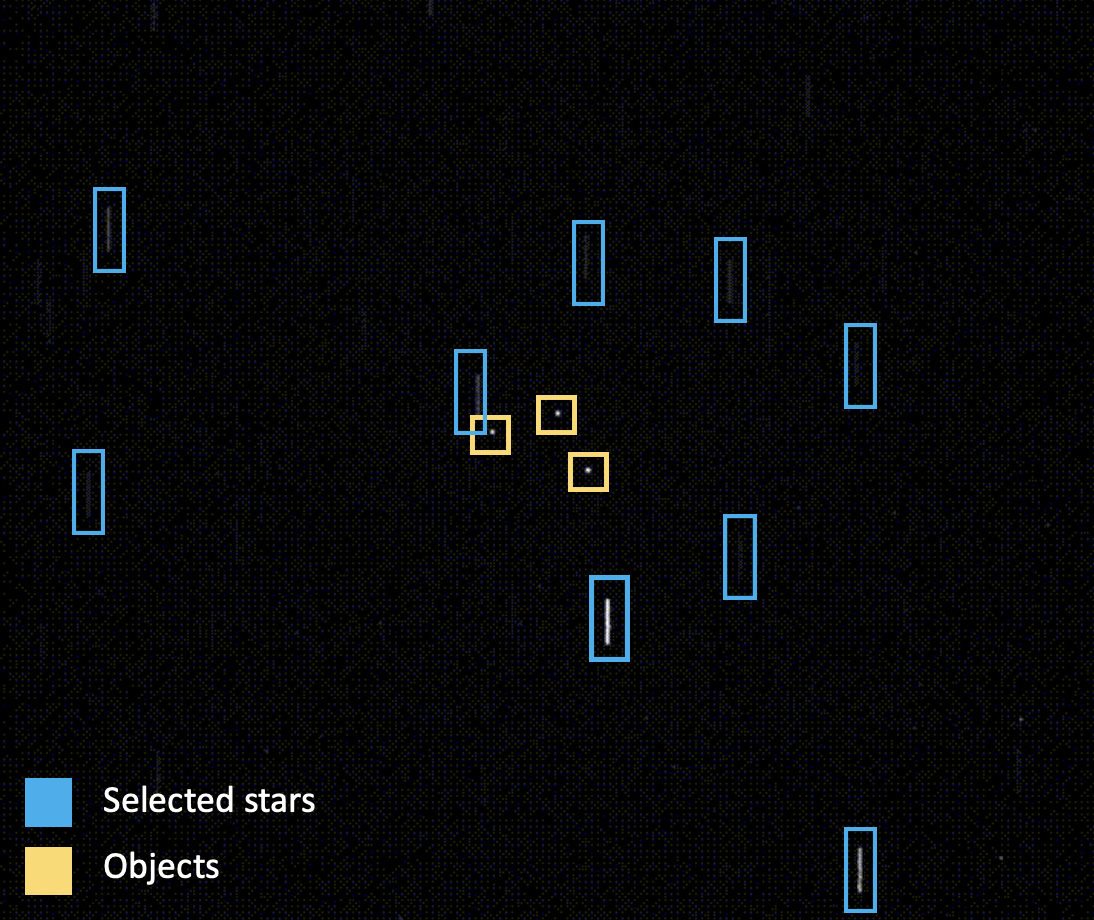
\includegraphics[width=\figmed]{static_images/static_pogs_annotated.png}
  \caption{Raw image of three GEO objects with stars streaking through the background. As expected the star signals have a variety of signal-to-noise ratios. Taken by the Purdue Optical Ground station at \pogslla by Nathan Houtz.}
  \label{fig:pogs_observation_example}
\end{figure}

Krag \cite{krag2003} modeled this signal by building a $1^\circ \times 1^\circ$ grid of surface
brightness values for the full inertial sphere, parameterized by RA/Dec. Krag used the
Guide Star catalog, which contains 15 million stars down to apparent magnitude 16. Exponential extrapolation
was used to predict star counts in each bin for higher magnitudes \cite{krag2003}. Twenty years later, larger star catalogs exist that are nearly complete to much higher apparent magnitudes. The integrated
starlight catalog used in this work was built from the GAIA catalog with approximately 1.5 billion
stars down to magnitude 21-22 \cite{gaia_dr3}. The same $1^\circ \times 1^\circ$ grid was computed
using GAIA \cite{astroquery_gaia}, resulting in Figure
\ref{fig:gaiapatched} which shows the computed brightness map in units of $S_{10}$. 

\begin{figure}[ht]
  \centering
  \includegraphics[width=\figbig]{sphx_glr_gaia_patched_catalog_001_2_00x.png}
  \caption{Integrated starlight brightness map}
  \label{fig:gaiapatched}
\end{figure}

With this map of exoatmospheric mean brightness of the night sky due to integrated
starlight, the corresponding signal mean in the telescope CCD is computed, adopting Krag's formulation \cite{krag2003}.

\begin{equation} \label{eq:bint}
 \textrm{BINT} = A_{aperture}
  \int_{10^{-8}}^{10^{-6}}{ \textrm{STRINT}(\lambda) \cdot \textrm{QE}(\lambda) \cdot \textrm{ATM}(\lambda)
  \cdot \left( \frac{\lambda}{h c} \right) \: d\lambda}  
\end{equation}

In Eq \ref{eq:bint}, $D$ is the telescope aperture diameter in meters, $h$ is Plank's constant in
$\left[ \frac{m^2 kg}{s} \right]$, and $c$
is the speed of light in vacuum in $\left[ \frac{m}{s} \right]$. The resulting quantity
$\textrm{BINT}$ has units of $\left[ \frac{1}{s} \right]$, representing the mean total photons passing
through the telescope aperture due to integrated starlight. 

\begin{equation} \label{eq:starlightmean}
  \bar{S}_{star} = 10^{-4} \cdot BINT \cdot \left( \frac{s_{pix}}{3600} \right)^2 \cdot \Delta t \cdot
  b_{is}
\end{equation}

In Eq \ref{eq:starlightmean}, $b_{is}$ is the integrated starlight brightness in $\left[ S_{10}
\right]$ computed by linearly interpolating the dataset in Figure \ref{fig:gaiapatched}, $s_{pix}$ is the telescope pixel scale in $\left[ \frac{arcsecond}{pix} \right]$, and $\Delta t$ is the integration time in seconds. Note the addition of the $10^{-4}$ factor to reconcile catalog surface brightness in terms of 10th magnitude stars, and the 0th magnitude source in $\textrm{BINT}$. This yields $\bar{S}_{star}$ with units $\left[ \frac{e^-}{pix^2} \right]$; photoelectron counts (ADU) per pixel. Figure \ref{fig:starlight_hemi} shows the background signal mean due to integrated starlight.

\begin{figure}[ht]
  \centering
  \includegraphics[width=\figmed]{sphx_glr_background_signals_002.png}
  \caption{Integrated starlight signal on the local observer hemisphere. The observer is in New Mexico, USA at
  \pogslla}
  \label{fig:starlight_hemi}
\end{figure}

\subsubsection{Scattered Moonlight}

Moonlight scattering through the atmosphere significant increases background brightness \cite{krag2003}. This scattering effect can be decomposed into Rayleigh (isotropically distributed) and Mie (exponentially distributed) scattering modes. The Rayleigh scattered component is computed with Table 4 published by Daniels parameterized by the angle from the observation to zenith $z_{obs}$, the angle from the Moon to zenith $z_{moon}$, and the angle between the observation and the Moon on the horizon $\Delta Az$ \cite{daniels1977}. Interpolating this table yields the intensity of the Rayleigh scattering $F_{rs}$ in $10^{-10}$ $W/(cm^2 \cdot \mu m \cdot sr)$ \cite{krag2003}. The Mie scattered component is formulated \cite{krag2003}:

\begin{equation} \label{eq:mie_scattering_moon}
  F_{ms}(\lambda) = a_1 \left[ e^{-\left(\frac{\Psi}{\Psi_1}\right)} + a_2 e^{-\left(\frac{\pi - \Psi}{\Psi_2}\right)} \right] F_{rs}(\lambda).
\end{equation}

Daniels recommends $a_1 \in [50, 100]$, $a_2 \in [0.01, 0.02]$, $\Psi_1 \in [10^\circ, 20^\circ]$, and $\Psi_2 \approx 50$ \cite{daniels1977}. Prior to any station-specific fitting, the middle of these intervals are chosen, yielding $a_1 = 75$, $a_2 = 0.015$, $\Psi_1 = 15^\circ$, and $\Psi_2 = 50^\circ$. $a_1$ and $a_2$ are dimensionless, such that $F_{ms}$ also has units of $10^{-10}$ $W/(cm^2 \cdot \mu m \cdot sr)$. The total intensity of the scattered moonlight $F_{mt}$ following Krag's formulation \cite{krag2003}:

\begin{equation} \label{eq:total_scattered_moonlight}
  F_{mt} = f(\theta) \left[ F_{rs}(\lambda) + F_{ms}(\lambda) \right].
\end{equation}

in Eq \ref{eq:total_scattered_moonlight}, $f(\theta)$ is the lunar phase function which describes the fraction of the full Moon brightness is reflected at an observer when the Sun-Moon-observer angle is $\theta$. This function is linearly interpolated within Table 3 in \cite{daniels1977}. Finally, Krag introduces a correction factor $f_{corr}$ to account for the difference between the Sun's irradiance spectrum and the spectrum of scattered moonlight, defined to be \cite{krag2003}:

\begin{equation} \label{eq:krag_f_corr}
  f_{corr} = \frac{I_0}{SUN(550 \: \left[\textrm{nm}\right])}.
\end{equation}

With all these pieces, the mean scattered moonlight signal in ADU per pixel is:

\begin{equation} \label{eq:moonlight_adu}
  \bar{S}_{moon} = F_{mt}(550 \: \left[\textrm{nm}\right]) \cdot SINT \cdot \left( \frac{s_{pix}}{3600} \right)^2 \cdot \Delta t \cdot f_{corr}.
\end{equation}

\begin{figure}[ht]
  \centering
  \includegraphics[width=\figmed]{sphx_glr_background_signals_001.png}
  \caption{Mean scattered moonlight signal on the local observer hemisphere. The observer is in New Mexico, USA at
  \pogslla}
  \label{fig:moonlight_hemi}
\end{figure}

\subsubsection{Zodiacal Light}

Zodiacal light is an effect created by sunlight reflecting off of dust in the ecliptic plane \cite{krag2003}. Zodiacal light is strongest around the Sun --- an exclusion zone for most optical telescopes --- but also reaches a peak directly away from the Sun due to the opposition effect. This peak is known as the Gegenschein, meaning "opposing light". The zodiacal light brightness is linearly interpolated within Table 1 of \cite{roach1972} which is listed for convenience in Appendix \ref{data:roach_zod}. This reports the surface brightness of the zodiacal light in $S_{10}$, which is used without conversion to find the mean CCD signal in ADU per pixel via:

\begin{equation} \label{eq:zodiacal_adu}
  \bar{S}_{zod} = BINT \cdot \left( \frac{s_{pix}}{3600} \right)^2 \cdot \Delta t \cdot ZOD \cdot 10^{-4}.
\end{equation}

As in the integrated starlight signal, the $10^{-4}$ factor reconciles the $S_{10}$ surface brightness with the 0th magnitude source in $\textrm{BINT}$. 

\begin{figure}[ht]
  \centering
  \includegraphics[width=\figmed]{sphx_glr_background_signals_004.png}
  \caption{Mean zodiacal light signal on the local observer hemisphere. The observer is in New Mexico, USA at
  \pogslla}
  \label{fig:zod_hemi}
\end{figure}

\subsubsection{Background Sampling}

The background signals are only defined in terms of their means, as each signal models the expected amount of radiation without accounting for the quantized nature of light \cite{krag2003}. Since light is transmitted in individual photons, their incidence on a given pixel will follow a statistical distribution. Assuming that each photon does not interact with others, the incidence of a photon on a pixel is well-modeled as a Poisson process for each background term \cite{frueh2019notes}. This distribution models the number of independent and identically distributed events that occur during a time period. For CCD astronomy, this translates to the event of a photon hitting the sensor. A Poisson distribution is defined on the positive integers by a single parameter $\lambda$ which is both the mean and variance of the distribution. The probability density function (PDF) for the Poisson distribution takes the form \cite{frueh2019notes}:

\begin{equation} \label{eq:poisson_pdf}
  P_\lambda(x=k) = \frac{\lambda^k e^{-\lambda}}{k!}.
\end{equation}

This distribution has a useful property that $P_{\lambda_1 + \lambda_2}(x=k) = P_{\lambda_1}(x=k) + P_{\lambda_2}(x=k)$ so long as the distributions described by $\lambda_1$ and $\lambda_2$ are independent. The background sources modeled in this work are reasonably assumed to be independent as they each originate from distinct physical processes.

\begin{equation} \label{eq:background_poisson}
  \lambda_{background} = \bar{S}_{airglow} + \bar{S}_{pollution} + \bar{S}_{twilight} + \bar{S}_{star} + \bar{S}_{moon} + \bar{S}_{zod}
\end{equation}

Drawing samples from the Poisson distribution defined by $\lambda_{background}$ computes the background of the CCD image. 

\subsection{Sensor Effects}

\subsubsection{Dark Noise}

The dark noise, also called the dark current or dark count, captures the temperature-dependent accumulation of electrons in the CCD pixel wells \cite{krag2003}. This noise source is modeled as a Poisson process with parameter $\lambda_{dark}$ \cite{frueh2019notes} and is assumed to be independent from the other sensor effects. This source accumulates with the integration time, giving it units of counts per second \cite{krag2003}.

\subsubsection{Readout Noise}

When the CCD is read out, the charge contained in each pixel well must be digitized. This process introduces noise in the final signal due to electronic effects within the CCD circuitry and its surrounding environment \cite{krag2003}. The readout noise is modeled as a zero-mean Gaussian distribution with variance $\sigma_{read}^2$ and is also assumed to be independent from other sensor effects \cite{frueh2019notes}.

\subsubsection{Truncation Noise}

Truncation noise in a CCD stems from the fact that the charge in each pixel is digitized into an integer factor of the gain \cite{frueh2019notes}. This is modeled using a uniform distribution on $\left[ -g/2, g/2 \right]$, yielding a variance $N^2_{trunc} = \frac{g^2}{24}$ \cite{frueh2019notes}.

The particular noise variances for the Purdue Optical Ground Station are listed in \ref{tb:pogs_parameters}.